\documentclass[preprint,12pt]{elsarticle}
\usepackage{graphicx}
\usepackage{amssymb}
\usepackage{amsmath}
\usepackage{hyperref}

\journal{COMP8230}

\begin{document}

\begin{frontmatter}

\title{Image Augmentation, A Marketing Approach}

\author{Reuben Francis}

\address{Macquarie University}

\begin{abstract}
The industry of digital marketing, fashion and advertising are in constant need of content creation., maybe a model posing for a luxury brand on a huge billboard or a suited-up woman for an interview opportunity online. This goes in hand with facial generation capabilities in the field of AI making huge leaps. Data Augmentation, a simple method can help create hyper-realistic images by synthesizing existing raw visual content, maybe from a renounced repository, facial stock photography or even loosely labeled Wikipedia images. We describe augmentation methods like generative adversarial networks and neural style transfer enriching an existing dataset with important facial appearance variations by manipulating the faces it contains, or changing a style of the image which help expand limited image datasets \cite{masi2016really}. The proposed method opens gates to industrial content automation and possibly even a hyper realistic fake model poses for a luxury clothing brand online \cite{DataGrid2019AI}. This in turn helps keep up with the ever-changing advertising trend, answer questions about its future ecosystem and sustenance in the digital world . 
\end{abstract}

\end{frontmatter}

\section{Industry context – Domain}
Image-based advertising has been around for a while, not just because it effectively helps understand messages into visual essence but also because visual over text-based messages is now the key drive for marketers’ target niche audiences. Just a few seconds between the advertiser and the customer needs to be enough to inspire a sentiment and leave an impression. This however required intelligent tools and resources and user experience which comes with a price to pay \cite{Ben2018}.
An understanding of dependencies on marketing industry helps realize the relentless need of data. Fashionable computer vision has become a long suit marketing tool \cite{WideEyes2017AI}, which however in terms of information gathering relies hugely on social media, places like Instagram, Pinterest and Tumblr requiring heavy feature extraction methods. Retail industry relies on digital marketing for product visibility to customers, this as an example requires a private data sharing source to the marketing agency, having no confidential information disclosed to anyone else.
Consumer behavior changes are now faster than companies can react. Data islands reside in media companies, private agencies or even open-sourced, however to protect the interests of advertisers, the ecosystem needs to come together and use powerful combination of data activation, a simple process of putting data stored in a data management system into action \cite{Maciej2016}

\section{Motivating Scenario}
\label{S:2}
It is now common knowledge how big brands are dependent on digital marketing for better reach, creating a new agency model that helps engineer brand experience and also better understand brand thinking and creativity. This requires intimate and immediate access to marketing data, which in context is very huge; display ads, social media ads, newspaper/magazines, event marketing, et cetera need relevant information that requires right data mining techniques, a classifier model needed to tag image well enough for label-based reproduction and other such analysis. The sheer volume of images, quick dynamic system approach, data island ownership and activation and ‘healthy’ data culture practice are some hardships that come in mind \cite{Mike2018}. 
Data-driven marketing is the future, with personalization, authenticity and relevance being perfected. This comes to the realization of computer vision compatibility which doesn’t just address said issues but helps add another perspective. The data availability is not always sufficient to define niche groups and meet needed goals, external open-sourced information is however available incorporating many useful facts. Augmenting this data would profit both company business value and customers with increased relevance \cite{Stef2019}.
Image augmentation, simply said is our motivating drive. Understanding data retrieval, extraction and augmentation techniques adds on to our motive which when realized resolves the issue of data scarcity. There sure is yottabytes of data present online but factors like company budget, poor data quality, data compatibility and data maintenance make it harder thereby explaining data scarcity .  Therefore, the idea of enriching existing image datasets with important feature variations exists, which helps resolve data-space solution without the worry of data availability. It is similar to imagination or dreaming, the techniques help ‘imagine’ what alterations are needed for an image.


\section{Problem Statement}
\label{S:3}
A good step to a change in the ecosystem is understanding the need to build a data-driven culture. A survey by Industry Index states that only 6\% of the ad industry is happy with the digital advertising ecosystem \cite{MCH2020}, with a conclusion that there needs to be an industry-wide standardization. There is quite a pool of problems to be discussed, marketers having difficulty getting a holistic view of customers across different data islands is one of the main challenges which can be tackled through customer behavior analytic platforms. Maintaining this system also helps ensure consistent experience throughout the customer life cycle. Being able to later tackle the lack of marketing expatriation helps personalize customer experience without violating privacy. This is a healthy data-driven approach but however our focus lies on other equally worrying customer-side marketing demands \cite{Mich2019dda}.
Difficulty tracking marketing effectiveness and media expenditure is concisely the grueling issue which in reality has definitely been tackled, this paper however tries using image (media) augmentation as a deep resolution, which in turn also helps tackle the lack of internal resources, precise attribution labelling and marketing technology integration problems \cite{Ross2019eMark}. This is solved by understanding the underlying issue of data availability. The overhead expenses are laid off by enriching existing data with better attribution knowledge and process of augmentation, the augmented data now becomes a valuable alternative or inclusion. 
In-image advertising is present everywhere whose popularity is gained by its ability to analysis past data, saved and shared images on different platforms and devices in real-time \cite{Steph2020advert}. This helps reach out to contextually-relevant users seamlessly viewing and sharing the content. These image recognizing ads however need to be able to analyze and access required data which isn't easy to centralize due to its sheer size. A company could rely on public use stock photography to save expense on hiring professional photographers for adverting needs but given our timeline requires a certain ‘de nos jours’ and as openly sourced as they could be, licensing issue exist \cite{Margot2019}. There tends to be a tendency of overuse and ‘cheesiness’, which rather can be solved when curated based on customer façade; realizing contextual and relevant facial feature extractions and human correction. In short, being able to change existing stock images with facial feature extractions or other image style transfers. 
Consider another scenario of a start-up e-commerce website using stock photography for web designing and relevant pop-up ad displays \cite{Ralitsa2019}. The amount of data that you have should be enough to personalize experiences to customers once you've taken over a buyer’s persona. Resource scarcity however limits the company to missed sale opportunity. Personalization using image augmentation helps create enriched images with existing ones. A stock image of a model wearing a certain piece of clothing can now have a different skin tone, expression, facial feature, chance to even have different colored clothing, or possibly even different clothing entirely, the choices are limitless.

\section{Approach}
\label{S:4}
Large scale commercial organizations have huge image datasets but none of these sets are publicly released. Downloading and labelling raw images is more than just a finance issue, it hinders personalization and creativity, this thereby demands the need to contribute with existing resources. Having realized the need to augment images, the required process however requires a lot of thought and detail. A great approach is synthesizing data in addition to limited collecting ability for data inflation \cite{book}.
There always exists an underlying assumption that more information can be extracted from a poorly sourced image. Simple transformations do exist where flipping, color spacing, cropping et cetera are a few options, this doesn’t however enrich data as to our needs \cite{Shorten2019ASO}. Some augmentation artificially manipulates existing images by making sure the labels are preserved, we use neural style transfer to do the needful. Some inflations however lead to oversampling, a good example of creating synthetic labels and thus giving multiple options which can be done by generative adversarial networks (GANs). Our oversampling technique also resolves class imbalance, crisis where a source might be scarce on a particular type of image when demanded. 

\subsection{GAN-based Image Augmentation}

Generative modeling popularly known as GANs are known for ‘unlocking’ information from data, this increased attention to how data augmentation could be applied. The architecture is a framework for generative modeling through adversarial training, a technique in machine learning that tries ‘fooling’ models through malicious input. The best way to understand GAN models is the cop versus counterfeiter analogy. The counterfeiter takes in any input and learns to produce money such that the cop cannot realize if it’s real or fake.  The counterfeiter takes the role of a generator network that takes in an image data and outputs desired ‘fake’, the cop serves as a discriminator network, able to distinguish between a real or generated image. The generator keeps trying until the discriminator cannot distinguish a generated image with a real one. The success of the generator to be able to fool a black-box discriminator system makes it very powerful. There are a lot of GAN architectures that exist through different network architectures, loss functions, et cetera being able to cater to said needs. The newly proposed StarGAN v2 \cite{choi2019stargan} model is a perfect image augmenter that helps resolve our problem statement mentioned before.   
Our augmenter works as an image-to-image translation model that needs to learn mapping different domains. A domain is identified as a group that’s visually distinguishable from others based on category. Each group however have images that are unique in how they appear, known as style. We consider gender as a domain with hairstyle, makeup, et cetera as styles. Being able to map these multi-domains is tedious and needs a unified framework to tackle scalability. A previous rendition, the StarGAN has a generator that takes image and domain label and transforms the image into said domain. It doesn’t however have a multi-modal system when it comes to its determinator. The StarGAN v2 replaces its domain labels with domain-specific style code which explains different styles for a specific domain. There exists a mapping network that learns to transform noise into style code and a style encoder that learns to extract style code from a given reference image. They have multiple branches for each domain which provides style code to the generator and therefore synthesizes images over multiple domains. 


\begin{figure}[ht]
\centering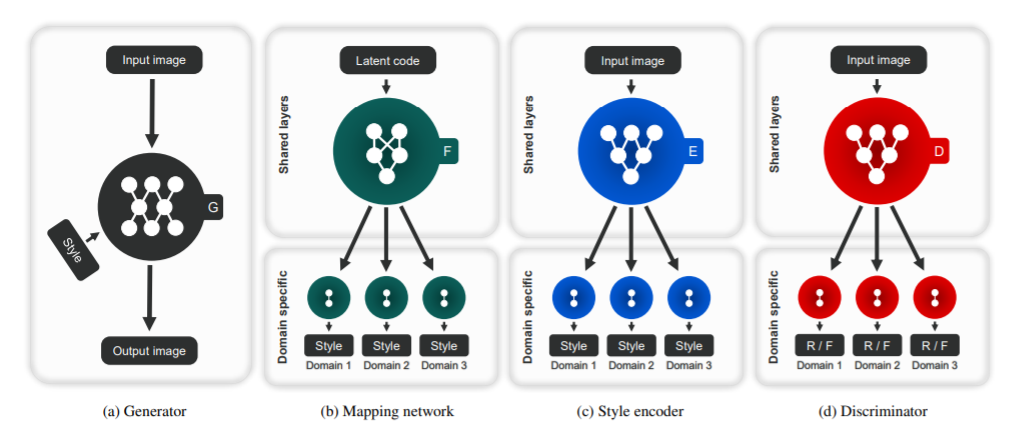
\includegraphics[width=1.0\linewidth]{starganv2.png}
\caption{Overview of StarGAN v2, consisting of four modules. (a) The generator translates an input image into an output image reflecting the domain-specific style code. (b) The mapping network transforms a latent code into style codes for multiple domains, one of which is randomly selected during training. (c) The style encoder extracts the style code of an image, allowing the generator to perform reference-guided image synthesis. (d) The discriminator distinguishes between real and fake images from multiple domains}
\label{fig:starganmodel}
\end{figure}



\subsection{Neural Style Transfer}

The basic idea of this technique is to manipulate how images from CNNs (Convolutional Neural Network) are represented, they are known to be very ‘flashy’ and are usually for artistic applications. They work by transferring the style of an image to another while keep true to its contents. We recognize the Fast Style Transfer by Gatys et al \cite{gatys2015neural} that uses a feed-forward network and a perceptual loss function, helps measure the ‘perceptual’ differences of the content and style image, they’re easier to understand as distance functions. We try to transform our content image while minimizing its content distance with itself and the style distance with the style image using backpropagation. The loss function comes through from another pre-trained net and shows super-resolution features. It also helps speed up style transfer, a great advantage for a practical use. The pre-trained image classification network VGG19 is the best example that we can use here, we can use its intermediate layers to define content and style feature representations.

\subsubsection{Content representation }
To understand content representations, we understand content distances mentioned before. The network is given the content image and an input image (initialized as the content image but is the one that is slowly generated) which returns the intermediate layer outputs, each iteration, a Euclidean distance is taken between the two intermediate representations of these images. 
The content loss is a function that calculates the distance of the content from the input image (x) and content image (p). Let C be the pre-trained deep convolutional neural network, therefore C(x) is the network given the image x. Let $F_{ij}^{l}(x)$ and $P_{ij}^{l}(p)$ (both belonging to C(x)) describe the respective intermediate feature representation of the network with input x and p at layer l of the ith filter at position j. The content loss is therefore defined as

\begin{equation}
L_{\text {content}}^{l}(p, x, l)=\frac{1}{2} \sum_{i j}\left(F_{i j}^{l}(x)-P_{i j}^{l}(p)\right)^{2}
\end{equation}

Backpropagation is performed such that it minimizes the content loss thus changing the input image (x) until it generates a similar response in a certain layer as the original content image (p). The reconstruction from lower layers is almost perfect while in the higher layers of the network, detailed pixel information is lost but the high-level features of the content image is preserved. This is the content representation. 

\subsubsection{Style representation}
Compared to content representation, it follows the same principle but instead we give the network an input image and style image. Instead of comparing the intermediate output layers, we instead compare the gram matrices of the input and style image. The style loss is the distance between the gram matrices of the input image (x) and the style image (a). Let $G_{ij}^{l}$ be the inner product between the feature maps i and j in layer l, this represents the correlation between the i and j feature maps.

\begin{equation}
G_{i j}^{l}=\sum_{k} F_{i k}^{l} F_{j k}^{l}
\end{equation}

To generate the style for input image we perform gradient descent (back-propagation) from the content image to transform it into image that represents the style of the original image. We minimize the mean square distance between the feature map of the style image and input image. Each layer contributes to the style loss which is represented by

\begin{equation}
E_{l}=\frac{1}{4 N_{i}^{2} M_{i}^{2}} \sum_{i j}\left(G_{i j}^{l}-A_{i j}^{l}\right)
\end{equation}

where $G_{ij}^{l}$  and $A_{ij}^{l}$  are the style representation in layer l of input image (x) and style image (a). $N_{i}$ is the number of feature maps, each of size $M_{i}$. The total style loss across each layer is

\begin{equation}
L_{\text {style}}(a, x)=\sum w_{l} E_{l}
\end{equation}

Here $w_{l}$ are the weighting factors of each layer to the total loss

\subsubsection{Style Transfer}
To transfer the style of an image (a) onto another image (p) we synthesize a new image that simultaneously matches the content representation of (p) and the style representation of (a). Here’s where the mentioned layers in the model creation are important, we minimize the distance of the feature representations of a white noise image from content representation of the one layer and style representation of the other image defined on the style layers. The loss function is now

\begin{equation}
L_{\text {total}}(p, a, x)=\alpha L_{\text {content}}(p, x)-\beta L_{\text {style}}(a, x)
\end{equation}

Here the $\alpha$ and $\beta$ are weighting factors for the content and style construction.

\begin{figure}[ht]
\centering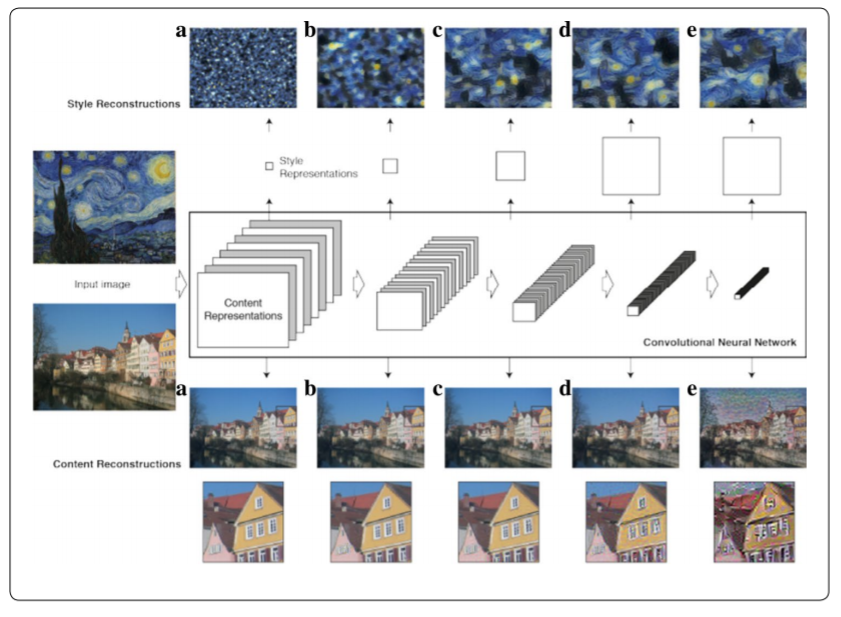
\includegraphics[width=0.7\linewidth]{nst.png}
\caption{Style and Content reconstruction in Neural Style Transfer}
\label{fig:nst}
\end{figure}

The need to create images with tons of ‘style’ images can be tempting, most papers use famous paintings and related abstract art to showcase how well the model works. A few applications might have obvious styles to transfer a content image based on the needs, but it usually isn’t that obvious. A recommended method for data augmentation is done by selecting a set of styles and applying them to all the required images, this also serves as a disadvantage since there’s effort needed to select styles for transfer.

\section{Results/Prototypes}
\label{S:5}
Having a good tool for image augmentation makes you realize as a visual marketer that you’re at a much better position to begin with, however knowing how to make full use makes you better. Our two models as examples of image augmentation help reach our goal of creating synthesized data, a quick resolve to marketing issues like data scarcity and ease of access to mention a few. As an ad agency trying to find relevance in this age, our GAN model requiring a source and reference image can be co-related to the agency figuring out a source image, a possible celebrity suddenly making rounds on social media could be a possible influence. A beard product consumer could be targeted required a bearded person as a reference. Scenarios like these encourage quick analysis of what source and reference could in turn not just help ‘increase’ in our choices but also exploit consumer behavior. A good example is our figure \ref{fig:stargan_result} showing a famous celebrity as a reference, a bearded male whose features have now been transferred to a few source images taken from CelebA-HQ dataset. Semantics such as hairstyle, makeup, beard and age are followed from the reference image, while pose and identity of the source remains the same. 

\begin{figure}[ht]
\centering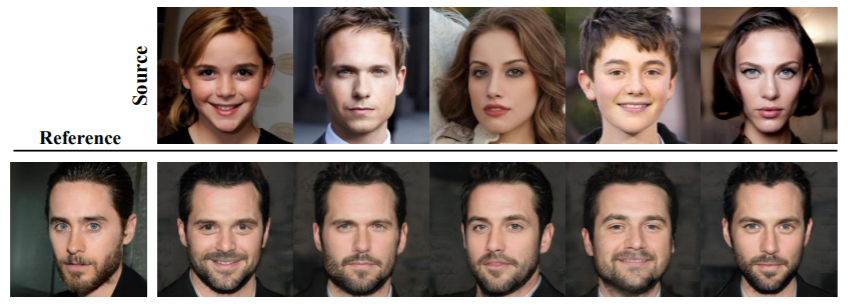
\includegraphics[width=0.7\linewidth]{stargan_result.png}
\caption{Reference-guided image synthesis results on CelebA-HQ. The source and reference images in the first row and the first column are real images, while the rest are images generated by our proposed model, StarGAN v2. Our model learns to transform a source image reflecting the style of a given reference image.}
\label{fig:stargan_result}
\end{figure}

The neural style transfer works on a similar basis, an image stays true to its contents however have a different style to them. A consumer in need of something ‘flashy’ could easily turn to NST for its nature. There are also ways in which adjusting weights adjust the balance of style and content representations. When synthesizing an image that combines the content of one image with the style of another, there usually does not exist an image that perfectly matches both constraints at the same time. The ratio of content weight ($\alpha$) and style weight ($\beta$) helps understand different variations of our styled image. Each most visually appealing image with a good balance of content and style can be tested out with our conventional models to see how they “react”.

\begin{figure}[ht]
\centering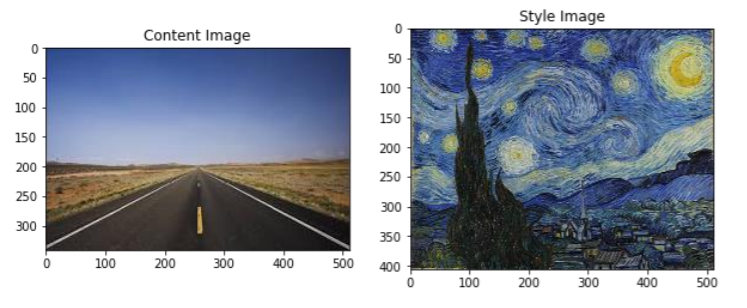
\includegraphics[width=0.7\linewidth]{content_style.png}
\caption{Example content and style image used for relative weighting}
\label{fig:content_style}
\end{figure}

A strong emphasis on style will result in images that match the appearance of the artwork, effectively giving a texturized version of it, but show hardly any of the image’s content. When doing the same on content, the style of the painting is not well matched and is almost unrecognizable. You would need to adjust the ratio of content and style to have a visually appealing image.

\begin{figure}[!h]
\centering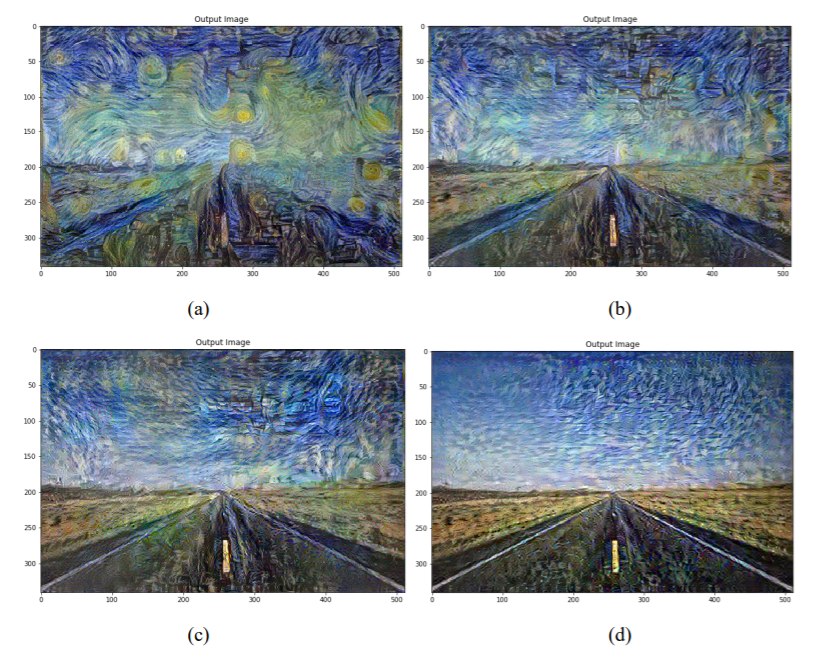
\includegraphics[width=0.5\linewidth]{relative_weight.png}
\caption{Relative weighting of matching content and style of the respective source images. The ratio $\alpha/\beta$ between matching the content and matching the style increases from top left to bottom right with (a) being $10^{-1}$ , (b) being $10^{2}$ , (c) being $10^{5}$, (d) being $10^{8}$}
\label{fig:relative}
\end{figure}

We can work on improving equality of losses by playing around with loss weights (possibly feature map size and filters) could help understand if we could give out a better image. It isn’t really easy to determine a “good” styled image. This is mostly because it is not clear what exactly defines the style of an image, our model struggles to understand what we truly need from the image to be represented onto the other, maybe it’s the brush strokes of the painting, the use of colors, the most dominant shapes that appear or possibly even just subjectively liking an image or a combination of all these factors.

\begin{figure}[!h]
\centering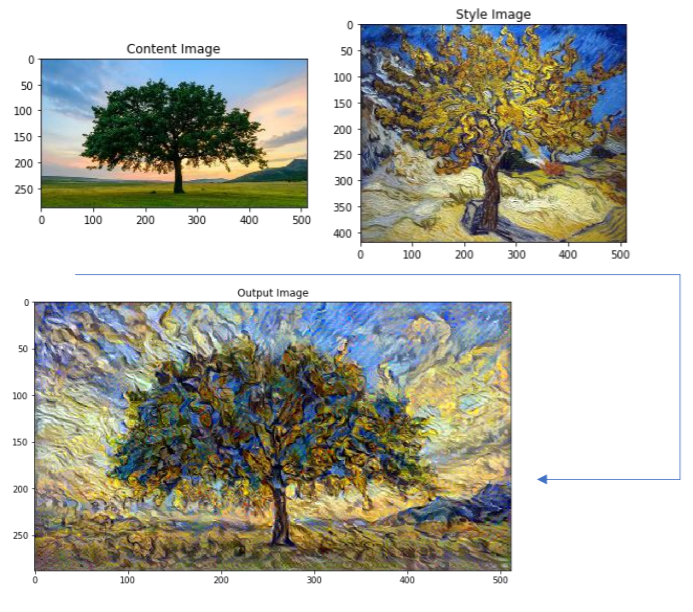
\includegraphics[width=0.7\linewidth]{nst_final.png}
\caption{The following example shows how the style image has some sort of correlation to the content image and therefore has some “purpose” to give an appealing styled image as an output.}
\label{fig:nst_final}
\end{figure}

\section{Conclusion}
\label{S:6}
There’s only 12\% of marketers that are currently using computer vision technology. Of these,  44\% use it to determine the reach of visual branding \cite{Ben2019Market}. The techniques mentioned work as prototypes for a bugger scenario, the marketing industry can use this evaluation or realization as a motivation for an industrial ready system. Image augmentation has still a long future along with computer vision. Our models serve as a baseline deep resolution to various open-ended solutions to advertisement or in that matter visual content creation in general. In-image ads have scope for content automation, a future where augmented images are automatically created for a said brand, based on customer interaction and other such analysis. 
The capability of GAN models can come to a point of being able to create hyper-realistic three-dimensional models, a good example is DataGrid’s fake fashion model Imma \cite{Mileva2019}. Instead of hiring new people every single time, brands can generate their own original content in a budget-friendly and efficient way. 

\begin{figure}[!h]
\centering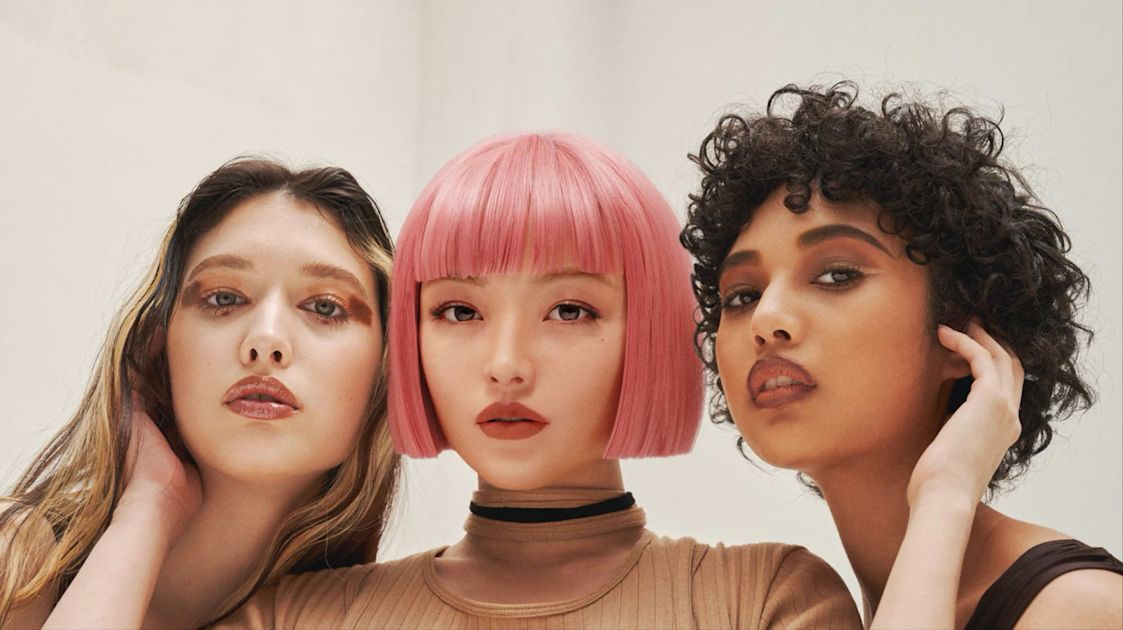
\includegraphics[width=0.7\linewidth]{dims.jpg}
\caption{DataGrid's fake model Imma [@imma.gram]}
\label{fig:imma}
\end{figure}

We are looking at a future where automation at a scale to operate, personalize, and enhance relationships becomes much more sophisticated and trusted by customers, this image creation technique opens doors to better ‘learning’ for said operations. Computer vision is also a case of interest in the fashion industry, our models might be limited but have a huge scope, the style transferring prototype is a perfect example of brand creativity for clothing. A system can have an opportunity to offer new styles for a specific dress for example. A possibility to forecast new fashion trend based on images it’s trained on and styled by. A future for virtual runways on digitally synthesized clothing and models \cite{Gum2017Fash}.  Customers responses on style preferences can directly be linked to our content-style based modelling of augmentation.  Marketing industry is just a focal point of discussion, the opportunities for our approach is still inherently expandable and still hasn’t been stepped on enough. 

\bibliographystyle{model1-num-names}
\bibliography{reference.bib}

\end{document}